\subsection{Finding a $t$-tough pair}\label{sec:gridfind}

Let $\calF$ be a relevant face of the skeleton $\Skel$ given by Lemma~\ref{lem:slicedskeleton}. If $F$ is the unbounded face of $\Skel$, then we change the embedding of $H_\Delta$ so that $F$ is not the outer face. Let $H^\calF$ denote the subgraph of $H$ induced by the vertices in $\calF$, and let $B$ denote the vertices that are on the boundary of $\calF$. We denote by $\bd \calF$ the edges of $H^\calF$ that are on the boundary of $\cal F$, and let $\inter \calF$ denote the edge set $E(H^\calF) \setminus \bd \cal F$. (Note that $\calF$ may contain undirected triangulation edges that are not contained in $\bd \calF$ or $\inter \calF$.) By Lemma~\ref{lem:slicedskeleton} we know that $\calF$ consists of $c_\Skel=O(1)$ segments. Observe that if we decompose the short segments on the boundary $\bd\calF$ into length-$0$ paths, then we can think of it as a collection of at most $L\cdot c_\Skel$ directed paths (where the long segments appear as themselves, and vertices only incident to short segments as singletons).

Given an (essential) edge $e$ in $\inter \calF$ (i.e., not on the boundary $\calF$), there exists a directed path in $H^\calF$ connecting two distinct vertices of $B$ using $e$ to satisfy the demand for which $e$ is essential. Note that the edges of this path are all in $\inter\calF$. Such a path is called an \emph{essential path} through $e$.

\begin{lemma}\label{lem:boundary_degree}
For each $v\in B$ we have that $\deg_{H^\calF}(v)\leq 2L\cdot c_\Skel+2$.
\end{lemma}

\begin{proof}
Let $vu$ be an edge where $v\in B$ and $u\not \in B$. Since $vu$ is essential for some demand, there is some essential path $P$ through $vu$; let $v'$ be the other endpoint of $P$. Suppose that $w'\in B$ is reachable from $v'$ along $\bd \calF$. Then there can be no essential path from $v$ to $w'$ that avoids $vu$, as the connection is already established by $P$ and the path along $\bd \calF$ from $v'$ to $w'$. In particular, there can be at most one edge leaving $v$ where the corresponding essential path ends on a given directed path of $\bd\calF$. Since $\bd\calF$ consists of at most $L\cdot c_\Skel$ directed paths, we have that there are at most $L\cdot c_\Skel$ inner edges leaving $v$. An analogous argument for the incoming edges plus the at most two boundary edges proves the desired upper bound on the degree of $v$.
\end{proof}

We will now consider the number of demands for which the edges of $H^\calF$ are essential. In what follows, let $\kappa$ be the number of such demands, i.e., suppose that $H\setminus \inter \calF$ fails to satisfy $\kappa$ of the demands.

\begin{lemma}\label{lem:essentials_intersectioncount}
If $H\setminus \inter \calF$ fails $\kappa$ demands, then the total branching degree of $H^\calF$ is at most $\kappa(\kappa-1)$.
\end{lemma}

\begin{proof}
First we show that the internal vertices of $H^\calF$ have bounded total branching degree. To do so, we first bound the number of intersections between paths satisfying different demands.

We claim that there can be at most one intersection point where there are incoming edges of $H^\calF$ essential for a given pair of demands. Suppose the contrary: that $v,w\in V(H^\calF)$ are distinct vertices such that both of them have an incoming edge essential for demand edge $d$ (denoted by $e(d,v)$ and $e(d,w)$ and an incoming edge essential for demand edge $d'$, denoted by $e(d',v)$ and $e(d',w)$. Note that either $v$ is reachable form $w$ or vice versa, as otherwise we could remove one of $e(d,v)$ and maintain the connection of $d$ via $w$. Assume without loss of generality that there is a path $P$ from $v$ to $w$. Note that $P$ cannot use both $e(d,w)$ and $e(d',w)$; suppose that it does not use $e(d,w)$.  Since $e(d,w)$ is essential for $d$, there is a directed path $Q\subset E(H^\calF)$ through it\footnote{Here $Q$ may use boundary edges of $H^\calF$, i.e., it is not necessarily an essential path.} satisfying the demand $d$. Note that $Q$ must also pass through the edge $e(d,v)$, and in particular, contains vertex $v$.

We can therefore use an initial part of $Q$ to get to $v$: note that this part of $Q$ is disjoint from $P$ as otherwise there would be a closed walk and thus a cycle in $H$. We use $P$ to go from $v$ to $w$, and continue on $Q$ after $w$; as $Q$ goes through $e(d,w)$, it can be continued from $w$. The resulting path $Q'$ essentially replaces $Q[v,w]$ with $P$, and has the same endpoints as $Q$, making $e(d,w)$ non-essential for $d$, a contradiction.

The analogous argument for outgoing edges gives the same bound. Imagine labeling each unordered pair of edges that have the same head with an unordered pair of demands, such that one edge is essential for one demand and the other edge is essential for the other. The above argument implies that these labels must be distinct for all pairs of edges sharing the same head. The analogous can be done for edge pairs that share the same tail. Consequently, the vertices of $H^\calF$ satisfy 
\begin{align*}
\sum_{v\in V(H^\calF)} \binom{\rho(v)}{2} &\leq \binom{\kappa}{2}\\
\sum_{v\in V(H^\calF)} \binom{\delta(v)}{2} &\leq \binom{\kappa}{2},
\end{align*}
where $\rho(v)$ and $\delta(v)$ denote the in- and outdegree of $v$ in $H^\calF$, respectively. On the other hand, observe that $\binom{\rho(v)}{2} + \binom{\delta(v)}{2} \geq d^*(v)$, thus we have that the total branching degree is at most $2\binom{\kappa}{2}=\kappa(\kappa-1)$.
\end{proof}

\begin{lemma}\label{lem:cbound_face_to_full}
If for each relevant face $\calF$ of $\Skel$ we have that $H\setminus \calF$ fails at most $\kappa$ demands, then, then the total branch degree of $H$ is at most $O(\kappa^2)\cdot k$.
\end{lemma}

\begin{proof}
By Lemma~\ref{lem:essentials_intersectioncount}, we have that each relevant face $\calF$ has total branch degree at most $\kappa(\kappa-1)$. Since each vertex of $H$ has degree at least $3$, the same holds for the vertices of $H^\calF$ that are in $\inter \calF$. Thus all of the inner vertices contribute at least $1$ to the branch degree of $H^\calF$; it follows that there are at most $\kappa(\kappa-1)$ inner vertices. It follows that the total degree of the inner vertices is at most $\kappa(\kappa-1)+2\kappa(\kappa-1)$, since the degree and branch degree differs by at most $2$. Let $B_\calF$ denote the vertices of $\bd\calF$, and let $\hat B_\calF$ denote those vertices that are adjacent to some inner vertex of $\calF$ in $H^\calF$. Since the total degree of inner vertices is at most $3\kappa(\kappa-1)$, this also bounds the number of vertices in $\hat B_\calF$: we have $|\hat B_\calF|\leq 3\kappa(\kappa-1)$.

By Lemma~\ref{lem:slicedskeleton} we know that $\Skel$ has $O(k)$ faces, thus the sum of the branch degrees of all relevant faces is $m=O(\kappa^2k)$. We claim that the total branch degree of $H$ is at most $O(k)$ larger than $3m$. Notice that the difference between the two amounts is due to the vertices of $H$ that lie on the shared boundary of some relevant faces of $\Skel$. Suppose now that $v$ has degree $2$ in $\Skel$ with neighboring relevant faces $\calF$ and $\calF'$. Then $d^*_H(v)\leq d^*_{H^\calF}(v)+d^*_{H^{\calF'}}(v) + 2$. Therefore, the total contribution from vertices in $\hat B_\calF$ is at most $2\kappa(\kappa-1)$, and all other vertices have all adjacent edges in the other face, so they satisfy $d^*_{\calF'}(v)=d^*_H(v)$.

Suppose now that $v$ has degree $d_v\geq 3$ in $\Skel$, with neighboring faces $\calF_1,\dots\calF_{d_v}$ and corresponding branch degrees $d^*_1(v),\dots, d^*_{d_v}(v)$. Then we have
\[ d^*_H(v)\leq \sum_{i=1}^{d_v} d^*_i(v) + 2(d_v -1).\]
Consequently, the branch degree of $\calH$ differs by at most $2\sum_v(d_v -1)$, where the sum goes over vertices of $\Skel$ of degree at least $3$. Note that $\Skel$ is a plane graph with $O(k)$ faces, thus the sum is at most $O(k)$, concluding the proof.
\end{proof}

We say that a directed edge $uv$ enters (resp. exits) a path $P$ if $u \not\in V(P)$ and $v\in P$ (resp. $u\in V(P)$ and $v\not\in V(P)$).

\begin{lemma}\label{lem:disjoint_essential}
Suppose that $P$ and $P'$ are essential paths for the edges $e,e'$ respectively, and that the directed paths $Q_s,Q,Q_t$ do not contain these edges. Suppose that $P$ and $P'$ exit the directed path $Q_s$ before $e$ and $e'$ respectively, and the edges $e,e'$ enter the same directed path $Q$. Alternatively, suppose that $e,e'$ exit the same directed path $Q$, and after them $P$ and $P'$ enter the same directed path $Q_t$. Then $P$ and $P'$ are vertex-disjoint, and the paths $Q_s,Q$ (respectively, $Q,Q_t$) have the same ``direction'', that is, their intersections with $P$ and $P'$ appear in the same order.
\end{lemma}

\begin{proof}
Let $e=uv$ and $f=u'v'$, and let $P$ and $P'$ be essential paths through $e$ and $f$ respectively, and suppose that $uv$ and $u'v'$ both enter a directed path. Let $Q$ denote the directed path from $v$ to $v'$. Let $s,t$ and $s',t'$ denote the start- and endpoints of $P$ and $P'$, respectively. We observe that the directed path $Q_s$ must be oriented from $s$ to $s'$: indeed, if it is oriented the other way, then $P'$ cannot be an essential path for $u'v'$, as we can use the path $s'\xrightarrow{Q_s} s\xrightarrow{P} v \xrightarrow{Q} v'$ instead of $P'[s',v']$, and we claim that this path avoids $u'v'$. In case of $Q_s$ and $Q$ do not contain $u'v'$, so one only needs to check $P$. But if $u'v'\in P[s,v]$, then we could create closed walk together with $Q$ and contradict acyclicity.

Now suppose for the sake of contradiction that $P$ and $P'$ intersect at some vertex $p$. We distinguish three cases:
\begin{description}
\item[Case 1:] $p$ occurs after the edge $uv$ on $P$.\\
This contradicts the essentiality of $uv$, as one can use $s\xrightarrow{Q_s} s' \xrightarrow{P'} p$ instead of $P[s,p]$.
\item[Case 2:] $p$ occurs before the edge $uv$ on $P$, and before the edge $u'v'$ on $P'$.\\
This contradicts the essentiality of $u'v'$, as one can use $p\xrightarrow{P} v \xrightarrow{Q} v'$ instead of $P'[p,v']$.
\item[Case 3:] $p$ occurs before the edge $uv$ on $P$, but after the edge $u'v'$ on $P'$.\\
This contradicts the acyclicity of $H$, as $p \xrightarrow{P} v \xrightarrow{Q} v' \xrightarrow{P'} p$ is a closed walk.
\end{description}


Suppose now that $uv$ and $u'v'$ both exit a directed path. Let $Q$ denote the directed path from $u$ to $u'$. We observe that the directed path $Q_t$ must be oriented from $t$ to $t'$: indeed, if it is oriented the other way, then $P$ cannot be an essential path for $uv$, as we can use the path $u \xrightarrow{Q} u'\xrightarrow{P'} t' \xrightarrow{Q_t} t$ instead of $P[u,t]$. Again this path avoids $uv$ as if $uv\in P'[u',t']$ then together with $Q$ we would get a closed walk. 

Now suppose for the sake of contradiction that $P$ and $P'$ intersect at some vertex $p$. We distinguish three cases:
\begin{description}
\item[Case 1:] $p$ occurs before the edge $u'v'$ on $P'$.\\
This contradicts the essentiality of $u'v'$, as one can use $p \xrightarrow{P} t \xrightarrow{Q_t} t'$ instead of $P'[p,t']$.
\item[Case 2:] $p$ occurs after the edge $u'v'$ on $P'$, and after the edge $uv$ on $P$.\\
This contradicts the essentiality of $uv$, as one can use $u \xrightarrow{Q} u' \xrightarrow{P'} p$ instead of $P[u,p]$.
\item[Case 3:] $p$ occurs after the edge $u'v'$ on $P'$, but before the edge $uv$ on $P$.\\
This contradicts the acyclicity of $H$, as $p \xrightarrow{P} u \xrightarrow{Q} u' \xrightarrow{P'} p$ is a closed walk.
\end{description}

This concludes the proof.
\end{proof}

A \emph{bundle} is a collection of pairwise vertex-disjoint essential paths of $\calF$ that exit a directed path $P_s$ of $\bd \calF$ and enter a directed path $P_t$ of $\bd\calF$. For a cycle $C$ in $\bar{H}^\calF_\Delta$ let $H^C$ denote the edges of $H$ that are inside\footnote{That is, in the fixed embedding, these edges lie entirely in the bounded region defined by $C$. Recall that all relevant faces of $\Skel$ are bounded.} $C$ or on $C$.

\begin{definition}[Grid structure]
A grid structure of size $\lambda$ is a cycle $C$ in $\bar{H}^{\calF}_\Delta$ and a pair of directed path sets $\calB_P = \{P_1,\dots,P_{\lambda}\}$ and $\calB_Q = \{Q_1,\dots,Q_\lambda\}$, where the paths are in $H^C$, and the following properties hold. See Figure~\ref{fig:griddef} for an illustration.
\begin{enumerate}[itemsep=1em,label=\textit{(\roman*)}]
\item Path $P_i$ starts at $s^P_i\in V(C)$ and ends at $t^P_i\in V(C)$. Similarly, path $Q_j$ starts at some $s^Q_j\in V(C)$ and ends at $t^Q_j\in V(C)$. Apart from their start- and endpoints, each $P_i$ and $Q_j$ is vertex-disjoint from $C$. The paths of $\calB_P$ are pairwise vertex-disjoint, and the paths of $\calB_Q$ are pairwise vertex disjoint.
\item The cycle $C$ contains the vertices
\[s^P_1,s^P_2,\dots,s^P_\lambda, \quad t^Q_1,t^Q_2,\dots,t^Q_\lambda, \quad t^P_\lambda,t^P_{\lambda-1},\dots,t^P_1, \quad s^Q_\lambda,s^Q_{\lambda-1},\dots,s^Q_1\]
in this cyclic order, or reversed.
\item There is a directed path $Q_s\subset C$ through $s^P_1,s^P_2,\dots,s^P_\lambda$. Similarly, the directed path $Q_t\subset C$ goes through $t^P_1,t^P_2,\dots,t^P_\lambda$, the path $P_s\subset C$ goes through  $s^Q_1,s^Q_2,\dots s^Q_\lambda$, and the path $P_t\subset C$ goes through $t^Q_1,t^Q_2,\dots,t^Q_\lambda$.
\item Each $P_i$ intersects each $Q_j$ in some non-empty connected subpath.
\item Each $P_i$ is a subpath of an essential path for some edge $e_i \in P_i$, and each $Q_j$ is a subpath of an essential path for some edge $e'_j \in Q_j$. Moreover, $e_i\not\in Q_j$ and $e'_j\not\in Q_i$ for any $i,j\in [\lambda]$.
\item For each $1\leq i_1<i_2\leq \lambda$ the head of $e_{i_2}$ is reachable from the tail of $e_{i_1}$ within $H^C$ using a path that avoids  $e_{i_1}$ or $e_{i_2}$. Similarly, the head of $e'_{i_2}$ is reachable from the tail of $e'_{i_1}$ within $H^C$ using a path that avoids  $e'_{i_1}$ or $e'_{i_2}$.
\end{enumerate}
\end{definition}

\begin{figure}[t]
\centering
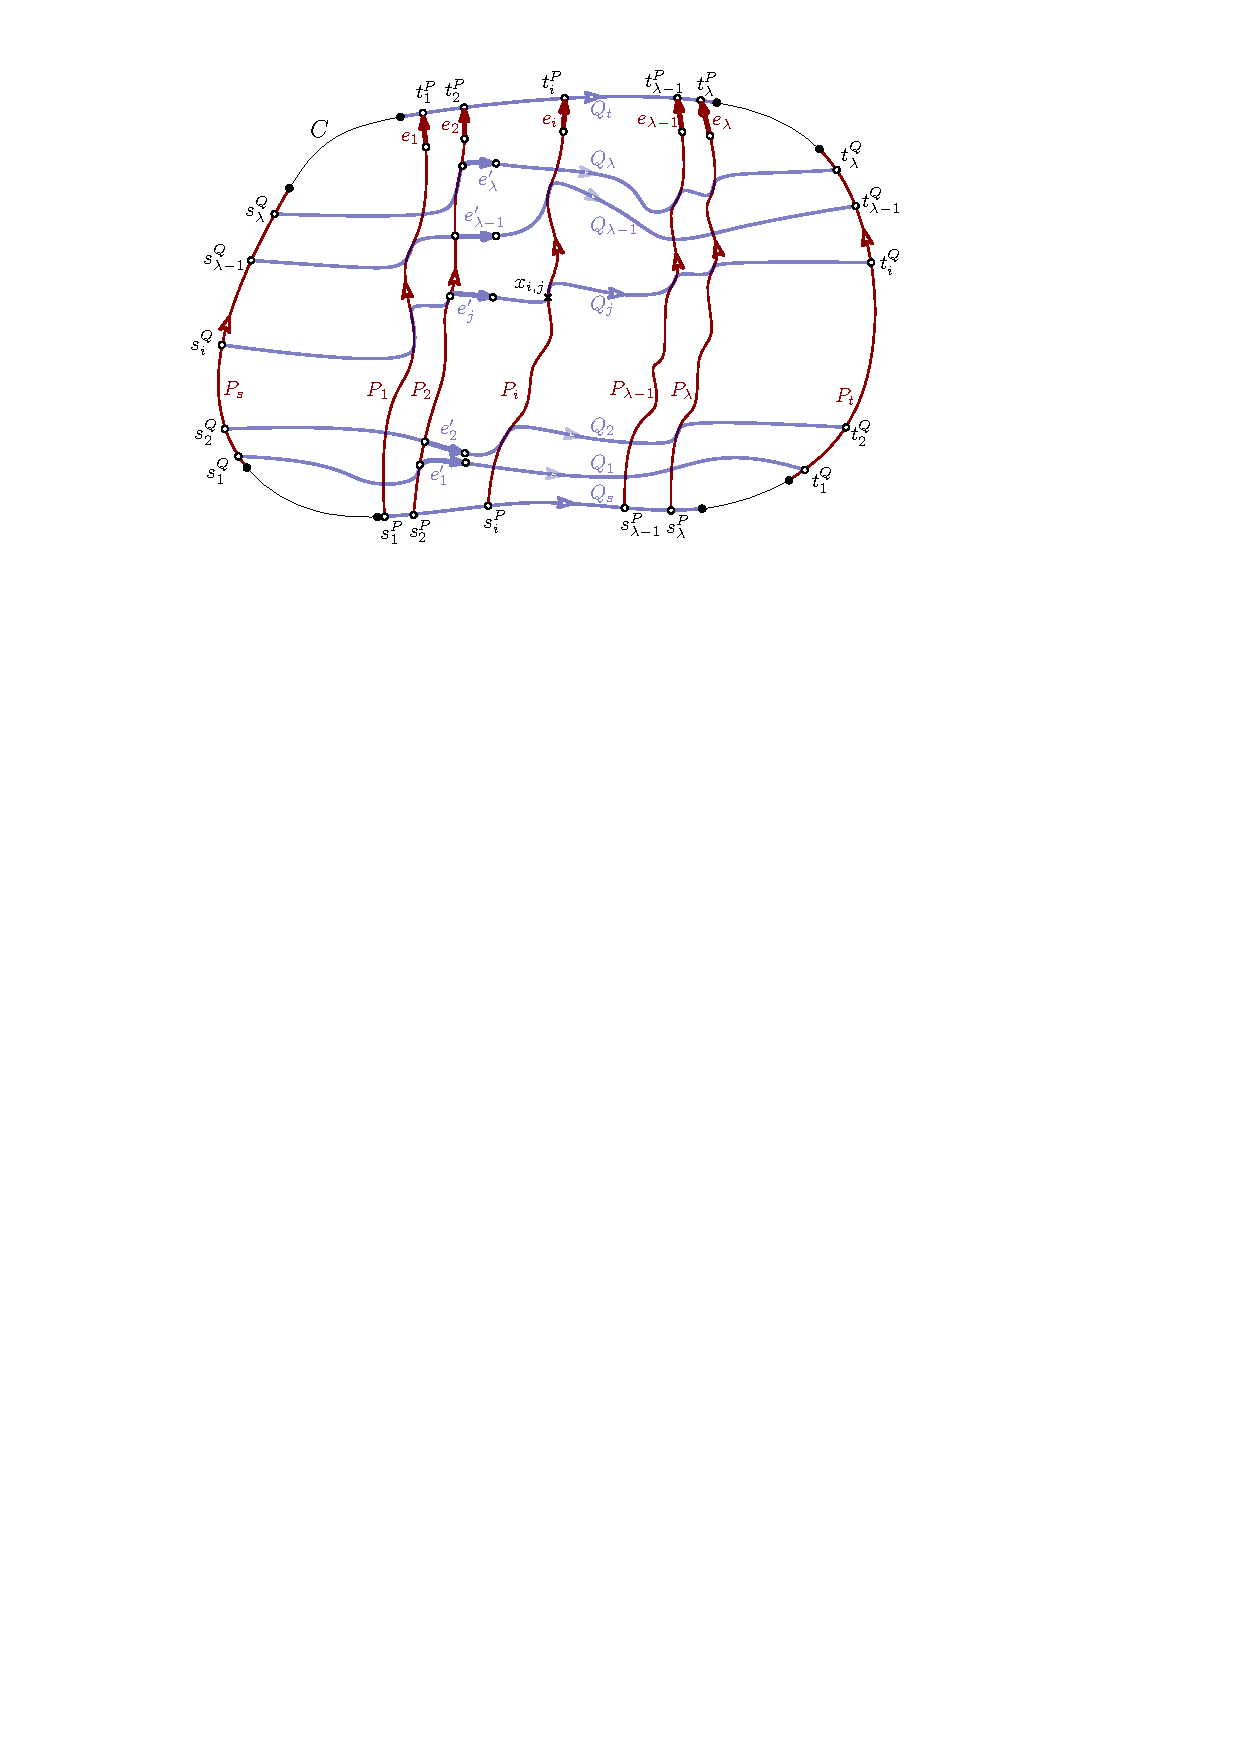
\includegraphics{griddef.pdf}
\caption{A grid structure with cycle $C$ and path sets $\calB_P,\calB_Q$. Thick edges are the defining essential edges. }\label{fig:griddef}
\end{figure}

Let us fix a vertex $x_{i,j}\in P_i\cap Q_j$ for each $i,j\in [\lambda]$. The embedding ensures that $x_{i,1},\dots,x_{i,\lambda}$ appear in this order on $P_i$, and $x_{1,j},\dots,x_{\lambda,j}$ appear in this order on $Q_j$. Observe that contracting the edges of $P_i\cap Q_j$ as well as all edges that have an incident degree-$2$ edge results in a plane grid with grid lines $P_i$ and $Q_j$.

Our task now is to find a large grid structure. Consider a bundle $\calB$ consisting of paths $P_1,\dots,P_t$ from long segment $A$ to long segment $B$ where the indices are according to the order of starting points on $A$. Suppose that $P_{t/4}$ starts at $a_1\in A$ and ends in $b_1\in B$, and that $P_{3t/4}$ starts at $a_2\in A$ and ends in $b_2\in B$. The \emph{spread} of $\calB$ is defined as $\dist_{\bar A}(a_1,a_2)+\dist_{\bar B}(b_1,b_2)$.

\begin{lemma}\label{lem:findgrid}
Suppose that $\kappa>L^4$ and that $L$ is large enough. If $H\setminus \inter \calF$ fails $\kappa$ demands, then $H^\calF$ has a grid structure of size $\Omega(L)$.
\end{lemma}

\begin{proof}
By Lemma~\ref{lem:boundary_degree} we have that each vertex on $\bd\calF$ has degree $O(Lc_\Skel)$. Since there are at most $Lc_\Skel$ vertices on $\bd \calF$ that are on some short segment, we have that at least $\kappa-O(L^2c^2_\Skel)$ demands whose essential paths go through long segments. Consequently, there exists a long segment $S$ that has $\frac{\kappa-O(L^2c^2_\Skel)}{c_\Skel}$ demands going through it. At least half of these demands are exiting $S$ or entering $S$; suppose the former, i.e., there are at least $\frac{\kappa-O(L^2c^2_\Skel)}{2c_\Skel}$ demands exiting $S$ (the entering case can be handled analogously). Since vertices of segment $S$ have degree at most $O(Lc_\Skel)$, we have that among these demands exiting $S$, there must be at least $\frac{\kappa-O(L^2c^2_\Skel)}{2c_\Skel\cdot O(Lc_\Skel)}=\Omega(\kappa/L)$ demands exiting $S$ that have pairwise distinct starting vertices.

Each of these demands have some edge exiting $S$, and for each of these edges let us fix a corresponding essential path. Among these essential paths, at most $O(L^2c^2_\Skel)$ of them end on short segments, and among the rest, at least $\frac{1}{c_\Skel}$ proportion of them end on the same long segment of $\bd\calF$. Thus there are at least 
$\frac{\Omega(\kappa/L)-O(L^2c^2_\Skel)}{c_\Skel}=\Omega(\kappa/L)$
essential paths among them that also end on the same long segment of $\bd \calF$. Among these paths, at least $\frac{1}{O(Lc_\Skel)}$ proportion of them have pairwise distinct ending points. Thus, there exists a bundle of size at least $\Omega(\kappa/L^2)$ where either all defining essential edges exit a long segment of $\bd \calF$, or all defining essential edges enter a long segment of $\bd \calF$. We fix a constant $c^*$ such that there exists a bundle of size at least $c^*\kappa/L^2$. Let $\calB$ be the bundle of minimum spread that has exactly $\lambda:=\lfloor L/(4c^2_\Skel)\rfloor$ and where the defining edges are all entering or all exiting a long segment.  Since $L$ is large enough, we may assume $L>1/c^*$, so $c^*\kappa/L^2>\kappa/L^3>L>\lambda$, so such a bundle $\calB$ exists.

By Lemma~\ref{lem:disjoint_essential}, we have that the paths of $\calB$ are pairwise vertex-disjoint. Moreover, by the same lemma, we can index  the paths of $\calB$ by the order in which their starting points occur in $\bd \calF$ as $P_1,\dots,P_\lambda$. By the essentiality of the defining edges of $\calB$, we know that the target of a path cannot be reachable from its source, thus the starting and ending long segments of $\calB$ are distinct and they cannot be subpaths of the same directed path of $H$. Thus Lemma~\ref{lem:slicedskeleton} implies that the starting and ending long segment of $\calB$ are distant, therefore there are at least $L$ vertices on the middle path $P_m$ of $\calB$, where we set $m=\lfloor \lambda/2 \rfloor$. Note that each vertex of $P_m$ has degree at least $3$, thus each of these vertices has an incident edge that is not on $P_m$. At least half of these edges are on the same side of $P_m$ in the embedding, and at least half of them are all entering or all exiting $P_m$. Consider now the essential paths of the $L/4$ edges selected this way. At least $1/c^2_\Skel$ proportion of them have the same starting and ending segment, thus there are at least $\lambda=\lfloor L/(4c^2_\Skel)\rfloor$ paths all entering or all exiting $P_m$ in the same direction. Let $\calB'$ be this size-$\lambda$ collection of essential paths.

We can index the paths of $\calB'$ by the order in which their essential edge occur on $P_m$ as $P'_1,\dots,P'_\lambda$. Let $e'_j$ the essential edge of $P'_j$.

Let $S_\calB, T_\calB, S'_\calB, T'_\calB$ be starting and ending segments of $\calB$ and $\calB'$, respectively. We denote by $e_i$ and $e'_i$ the essential edge of $P_i$ and $P'_i$. Suppose now that $P_i$ and $P'_j$ intersect more than once, and let $x$ and $x'$ be the first and last intersection along $P_i$. By acyclicity of $H$, we know that $x$ and $x'$ are also the first and last intersection along $P'_j$. Observe that the $e_i$ and $e'_j$ cannot occur between $x$ and $x'$, as that would allow us to circumnavigate an essential edge using a portion of the other path. Consequently, we can change $P'_j$ by exchanging $P'_j[x,x']$ with $P_i[x,x']$; the result is still an essential path for the edge $e'_j$. By making such changes exhaustively, we can ensure that for each $i,j\in [\lambda]$ if $P_i$ intersects $P_j$, then their intersection is a connected (possibly one-vertex) subpath. 

We now distinguish several cases based on what segment $\calB'$ starts and ends on.  Note that $S_\calB\neq T_\calB$ and $S'_\calB\neq T'_\calB$ by essentiality of $e_1$ and $e'_1$, and acyclicity. Assume without loss of generality that $\calB$ goes from bottom to top, with both $S_\calB$ and $T_\calB$ oriented left to right. See Figure~\ref{fig:findgrid}	 for an illustration.


\paragraph*{Case 1.} $S'_\calB\not\in \{S_\calB,T_\calB\}$ (or symmetrically, $T'_\calB\not\in \{S_\calB,T_\calB\}$).
First we show that the paths of $\calB'$ are pairwise disjoint. Suppose that the edges $e'_j$ are entering $P_m$ from the left. Then we can apply Lemma~\ref{lem:disjoint_essential} with $P_1$ playing the role of $Q_s$ and $P_m$ playing the role of $Q$.  If they are exiting $P_m$ on the right, and $T'_\calB \not\in \{S_\calB,T_\calB\}$, then Lemma~\ref{lem:disjoint_essential} is applied with $Q=P_m$ and $Q_t=P_\lambda$. If $T'_\calB \in \{S_\calB,T_\calB\}$, then Lemma~\ref{lem:disjoint_essential} is applied with $Q=P_m$ and $Q_t=T'_\calB$. All remaining cases can be handled with analogous invocations of Lemma~\ref{lem:disjoint_essential}.

Suppose that the edges $e'_i$ enter $P_m$ from the left or exit it on the right. Because of the embedding it follows that all paths of $\calB'$ intersect $P_1,P_2,\dots,P_m$. We claim that if the edges $e'_i$ exit $P_m$, then the paths $P'_i$ also intersect the path $Z=S_\calB[m,m+1]\cup P_{m+1}$, where $S_\calB[m,m+1]$ denotes the portion of $S_\calB$ between the starting point of $P_m$ and $P_{m+1}$. Note that $P'_i$ enters the inside of the closed curve $P_{m} \cup S_\calB[m,m+1] \cup P_{m+1} \cup T_\calB[m,m+1]$, so $P'_i$ must intersect $Z$ or $T_\calB[m,m+1]$ after passing $e'_i$ (because of the earlier simplifaction it cannot intersect $P_m$ again). If $P'_i$ enters $T_\calB[m,m+1]$, then its portion containing $e'_i$ can be curcumnavigated on a directed subpath of $P_m\cup T_\calB[m,m+1]$, contradicting the essentaility of $e'_i$.

If $e'_i$ enters $P_m$, then we set $Z=P_m$.

Consider the cycle $C$ of $\bar H$ formed by $P_1,P'_1,P'_m,Z$ (Since $P_1,Z$ and $P'_1,P'_m$ are vertex-disjoint, and the other pairs have a connected intersection, there is a unique cycle in the union $P_1 \cup P'_1 \cup P'_m \cup Z$.) One can verify that $C$, $\{P_2|_C,\dots,P_{m-1}|_C\}$, and $\{P'_2|_C,\dots,P'_{m-1}|_C\}$ form a grid structure, where $P|_C$ denotes the portion of the path $P$ that falls in the interior of the bounded region of $C$.

The case when the edges $\calB'$  enter $P_m$ from the right or exit it to the left can be handled analogously, using the paths $P_m,\dots,P_\lambda$ instead of $P_1,\dots, P_m$, and setting $Z=P_{m-1}\cup T_\calB[m-1,m]$ or $Z=P_m$ for entering/exiting edges $e'_i$. The cycle $C$ is defined by $Z,P_\lambda,P'_m,P'_\lambda$, and the grid is given by $C$, $\{P_{m+1}|_C,\dots,P_{\lambda-1}|_C\}$, and $\{P'_{m+1}|_C,\dots,P'_{\lambda-1}|_C\}$. In all cases the grid has size at least $\lfloor \lambda/2 \rfloor -2$.

\begin{figure}[t]
\centering
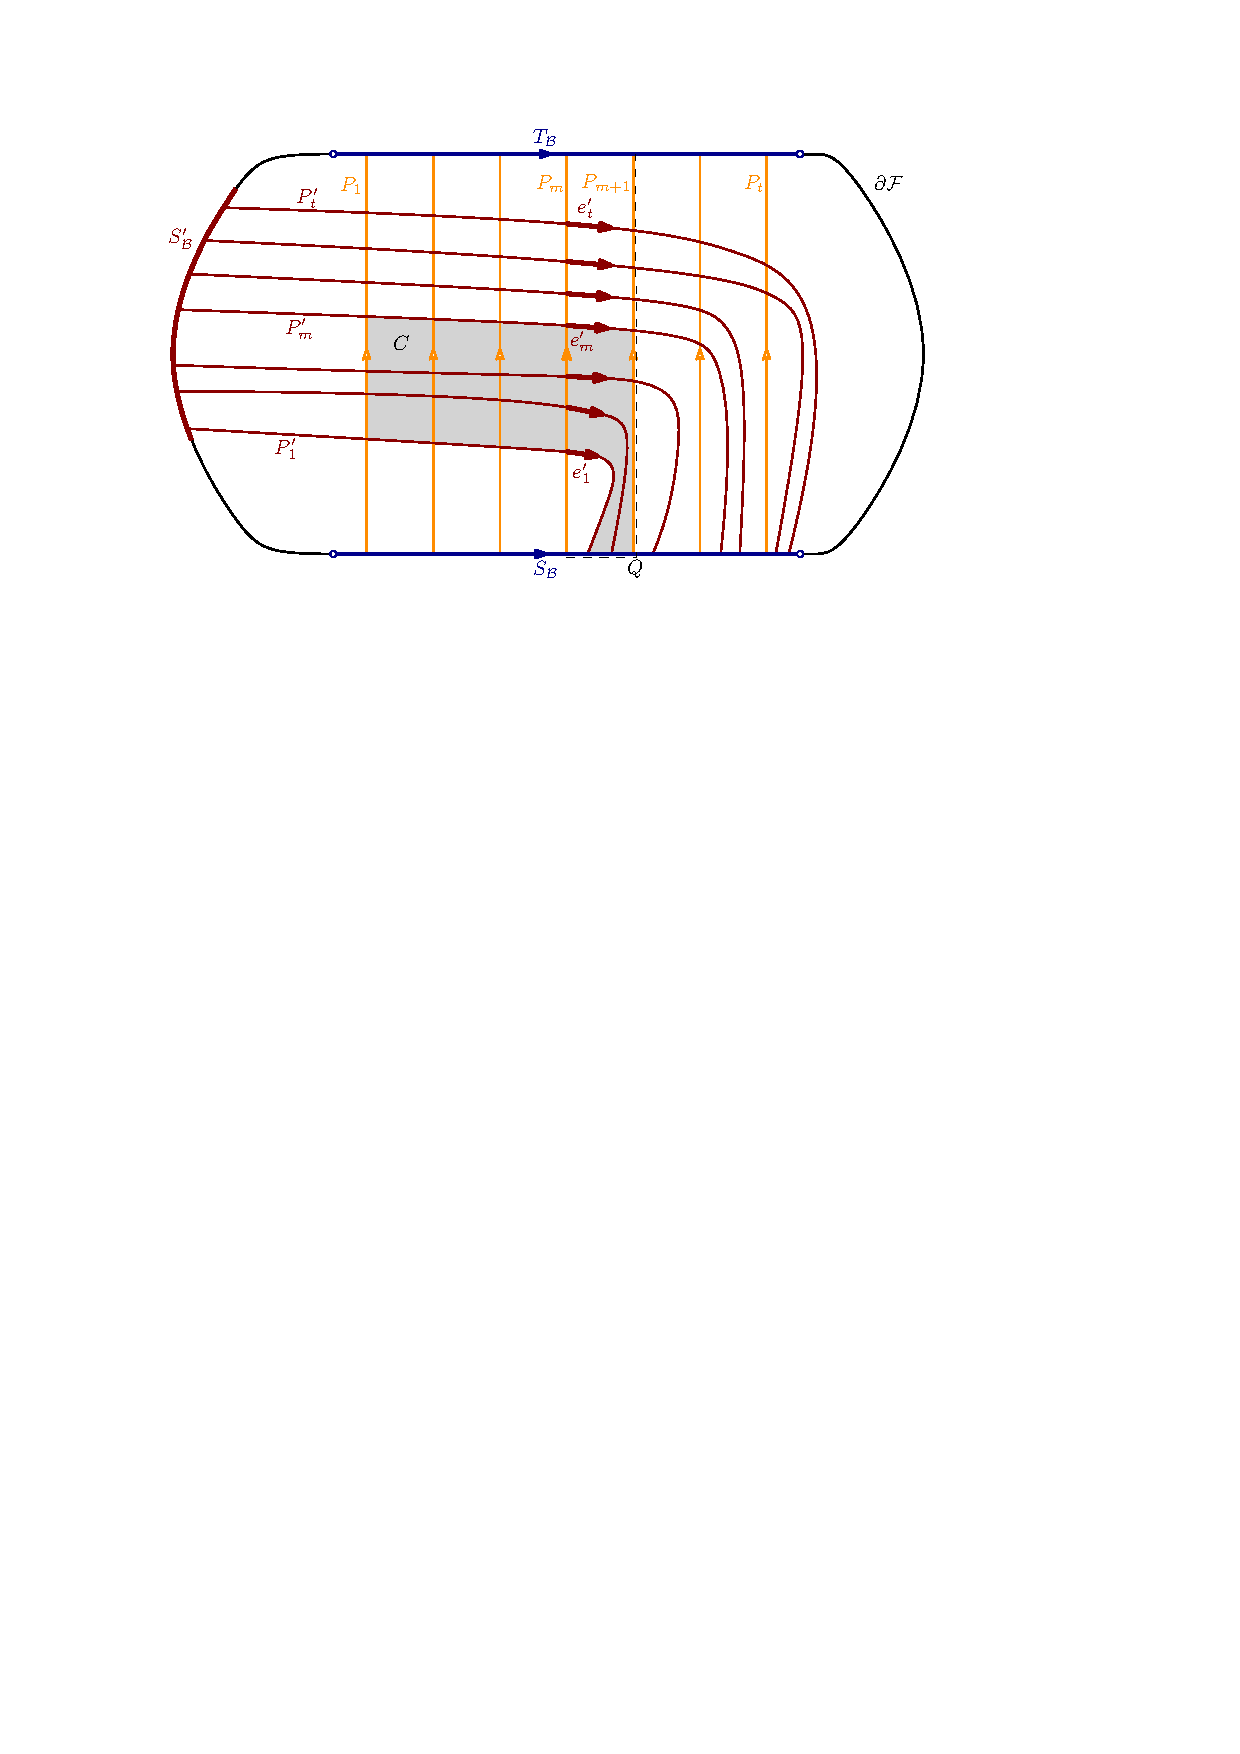
\includegraphics{findgrid.pdf}
\caption{Finding a grid structure based on a bundle $\calB$ (orange). The edges $e'_j$ exit the middle path $P_m$ on the right. The bundle $\calB'$ (red) has a distinct starting segment $S'_\calB$, as in Case 1. The directed path $Z$ is depicted with dashed line, and the cycle $C$ around the found grid is the boundary of the gray shaded region.}\label{fig:findgrid}
\end{figure}

\paragraph*{Case 2.} $S_\calB=S'_\calB$ and $T_\calB=T'_\calB$. We claim that this case cannot occur.
If $e'_i$ exits $P_m$ on the right, then we can exchange the portion of $P'_i$ starting at $e'_i$ with a part of $P_m$ and $T_\calB$, contradicting the essentiality of $e'_i$. If $e'_i$ enters $P_m$ from the left, then we can exchange the portion of $P'_i$ ending at $e'_i$ with a part of $S_\calB$ and $P_m$, contradicting the essentiality of $e'_i$.

If $e'_i$ exits $P_m$ on the left, or enters $P_m$ from the right, then we can exchange the portion of $P_m$ starting at $e_m$ with a part of $S_\calB$ and $P'_m$, contradicting the essentiality of $e_m$.

\paragraph{Case 3.} $S_\calB=T'_\calB$ and $T_\calB=S'_\calB$.
First we note that $e'_i$ cannot enter $P_m$ from the right or exit it on the left, as both would create a cycle. We can invoke Lemma~\ref{lem:disjoint_essential} on any pair of paths of $\calB'$ with $Q=P_m$ and either $Q_s=S'_\calB$ or $Q_t=T'_\calB$ to prove that the paths of $\calB'$ are pairwise vertex-disjoint.

Since $\calB$ has minimum spread, we have that $\calB'$ has a spread at least as big. Recall that if $\calB$ goes from $A=S_\calB$ to $B=T_\calB$, then $P_{\lambda/4}$ starts at $a_1\in A$ and ends in $b_1\in B$, while $P_{3\lambda/4}$ starts at $a_2\in A$ and ends in $b_2\in B$. Now $\calB'$ goes from $B$ to $A$, so we set the start and endpoint of $P'_{\lambda/4}$ as $b'_1\in B$ and $a'_1\in A$, and similarly, the start and end of $P'_{3\lambda/4}$ as $b'_2\in B$ and $a'_2\in A$. Now $\dist_{\bar A}(a_1,a_2)+\dist_{\bar B}(b_1,b_2) \leq \dist_{\bar A}(a'_1,a'_2)+\dist_{\bar B}(b'_1,b'_2)$, thus at least one of the inequalities $\dist_{\bar A}(a_1,a_2) \leq \dist_{\bar A}(b'_1,b'_2)$ and $\dist_{\bar B}(b_1,b_2) \leq \dist_{\bar B}(a'_1,a'_2)$ holds.

Suppose that the latter inequality holds. Then because of the embedding we have that $P'_1,\dots,P'_{\lfloor \lambda/4\rfloor}$ all intersect $P_{\lceil \lambda/4 \rceil},\dots, P_{\lfloor \lambda/2 \rfloor}$. We can then define a grid for these two smaller bundles of size at least $\lambda/4-2$ as seen in Case 1 by imagining that the path $T_\calB$ is split into two shorter paths, the first part containing the endpoints of $P'_1,\dots,P'_{\lfloor \lambda/4\rfloor}$, and the second containing the starting points of $P_{\lceil \lambda/4 \rceil},\dots, P_{\lfloor \lambda/2 \rfloor}$. Similarly, if the former inequality ($\dist_{\bar B}(b_1,b_2) \leq \dist_{\bar B}(a'_1,a'_2)$) holds, then $P'_{\lceil 3\lambda/4 \rceil},\dots,P'_{\lambda}$ all intersect $P_{\lceil \lambda/2 \rceil},\dots, P_{\lfloor 3\lambda/4 \rfloor}$, and the grid can again be defined analogously to Case 1.\\

In all possible cases we have shown that a grid of size $\Omega(\lambda)=\Omega(L)$ exists which completes the proof.
\end{proof}

The usefulness of the grid structure is demonstrated by the following lemma.

\begin{lemma}\label{lem:gridsarehard}
If $C,\calB$, and $\calB'$ form a grid structure of size $\lambda$, then the demands corresponding to a subset of their essential paths form a  $(\lambda-2)$-tough pair.
\end{lemma}

\begin{proof}
First we show that the demands corresponding to the essential paths $\calB_P=\{P_1,\dots,P_\lambda\}$ are pairwise weakly independent. For a path $P_i$ let $d^P_i=u^P_iv^P_i$ be the corresponding minimal demand, which is served by some path $P^{ex}_i$ that is an extension of $P_i$. (Similarly, the minimal demand of $Q_j$ is $d^Q_j=u^Q_jv^Q_j$, and it is served by the path $Q^{ex}_j$.) See Figure~\ref{fig:findtough} for an illustration.

Suppose now that $d^P_i$ and $d^P_j$ are not weakly independent, where $i<j$. There cannot be a demand $v^P_ju^P_i$, as a path satisfying this demand together with $P^{ex}_i[u^P_i,x_{i,1}]\cup Q_1[x_{i,1},x_{j,1}] \cup P^{ex}_j[x_{j,1},v^P_j]$ forms a closed walk, i.e., contradicts acyclicity. Thus weak independence must be violated by a demand $v^P_iu^P_j$; let $P_d$ be the path corresponding to this demand. We claim that this contradicts the essentiality of $e'_2$, as $Q^* = Q_2[s^Q_2,t^Q_2]$ can be exchanged with the path
\[P^* = s^Q_2 \xrightarrow{P_s} s^Q_3 \xrightarrow{Q_3} x_{i,3} \xrightarrow{P^{ex}_i} v^P_i \xrightarrow{P_d}
u^P_j \xrightarrow{P^{ex}_j} x_{j,1} \xrightarrow{Q_1}  t^Q_1  \xrightarrow{P_t} t^Q_2.\]

\begin{figure}[t]
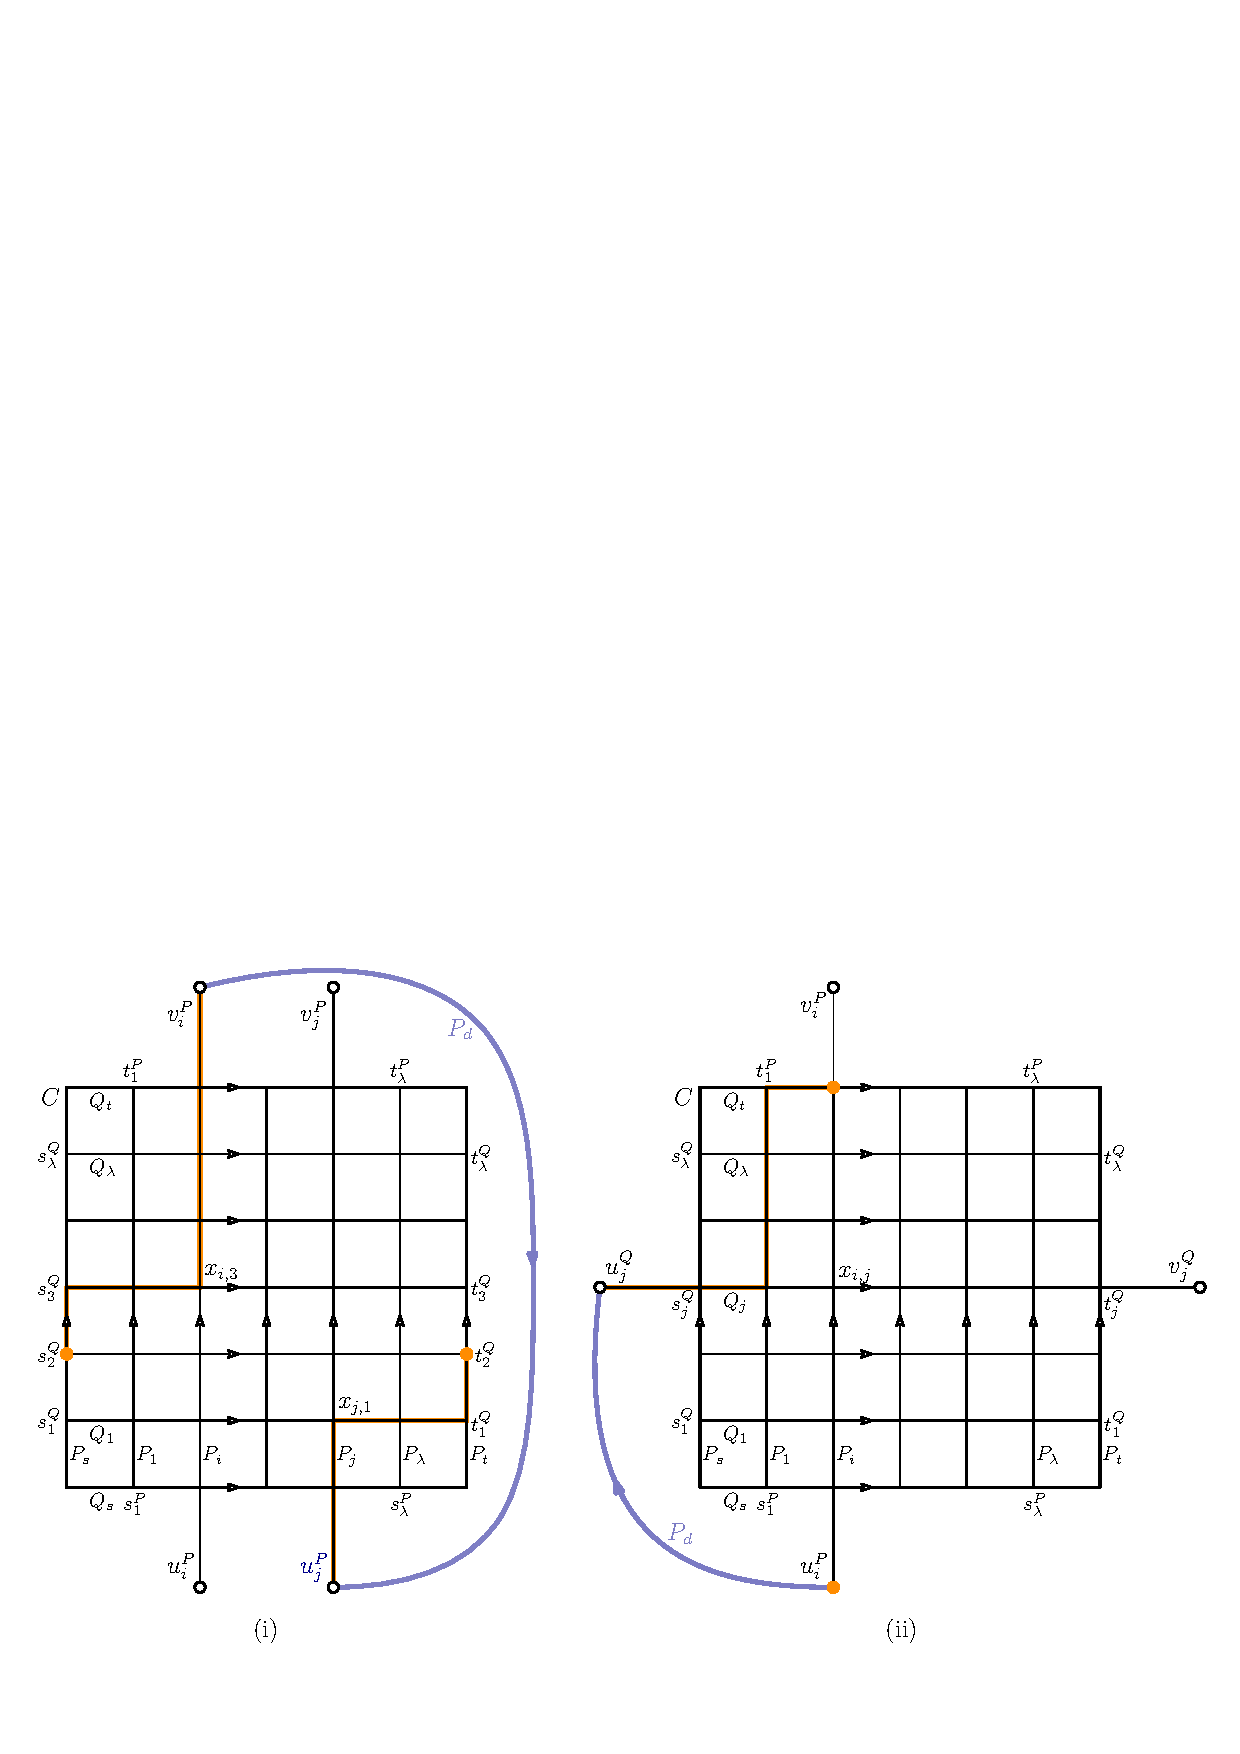
\includegraphics[width=\textwidth]{findtough.pdf}
\caption{(i) Proving weak independence: a demand $v^P_i u^P_j$ leads to the path $Q_2$ being avoidable, contradicting essentiality of $e'_2$. (ii) Proving strong independence. A demand $u^P_iu^Q_j$ leads to the edge $e_i$ being avoidable on $P^{ex}_i$, contradicting its essentiality for $u^P_iv^P_i$. In both sides the path $P^*$ is represented as the concatenation of the path(s) with orange background and the blue path~$P_d$.}\label{fig:findtough}
\end{figure}

Unless $P^*$ also contains $e'_2$, this exchange contradicts the essentiality of $e'_2$.
Suppose now that $P^*$ does contain $e'_2$; by the properties of the grid we know that $e'_2$ cannot lie on any of $P_s,Q_3,P^{ex}_i,P^{ex}_j,Q_1,P_t$, thus it could only be contained in $P_d$. Notice that if $e'_2$ is not essential for the demand of $P_d$, then we can change $P_d$ to exclude $e'_2$ and get a contradiction as above. Thus in what follows, we assume that $e'_2$ is an essential edge for $P_d$.

Notice that the same argument can be repeated for $e'_3$, thus $P_d$ must contain $e'_3$ as an essential edge. By Property (vi) of grid structures, the head of $e'_3$ is reachable from the tail of $e'_{2}$. It follows that $e'_2,e'_3$ must appear in this order on $P_d$, as otherwise we could create a closed walk ($\tail(e'_2) \rightarrow \head(e'_3) \xrightarrow{P_d} \tail(e'_2)$), contradicting acyclicity. Consequently, $P_d$ has a subpath \[\tail(e'_2) \xrightarrow{e'_2} \head(e'_2)\xrightarrow{P_d} \tail(e'_3) \xrightarrow{e'_2} \head(e'_3),\] which we could replace with the guaranteed path $\tail(e'_2) \rightarrow \head(e'_3)$ from the grid structure that avoids $e'_2$ or $e'_3$, contradicting the essentiality of either $e'_2$ or $e'_3$ for $P_d$.
The weak independence of the paths $Q_j$ can be proven symmetrically (by switching the role of $P$ and $Q$).

Next we show strong independence of $d^P_i$ and $d^Q_j$ for all $i,j\in \{2,3,\dots,\lambda-1\}$. Notice that this is sufficient, as it shows that the demands $d^P_2,\dots,d^P_{\lambda-1}$ and $d^Q_2,\dots,d^Q_{\lambda-1}$ form a $(\lambda-2)$-tough pair. Observe that having a demand $v^Q_ju^P_i$ or $v^P_iu^Q_j$ for any $i,j$ would create a closed walk:
\[
x_{i,j} \xrightarrow{Q^{ex}_j} v^Q_j \xrightarrow{} u^P_i \xrightarrow{P^{ex}_i} x_{i,j} \quad
\text{ and } \quad
x_{i,j} \xrightarrow{P^{ex}_i} v^P_i \xrightarrow{} u^Q_j \xrightarrow{Q_j} x_{i,j},\]
respectively, contradicting acyclicity.
Suppose now that there is a demand $u^P_iu^Q_j$ served by a path $P_d$, where $i,j\in \{2,3,\dots,\lambda-1\}$. Then the path $P^{ex}_i[u^P_i, t^P_i]$ can be replaced by
\[P^*=u^P_i \xrightarrow{P_d} u^Q_j \xrightarrow{Q^{ex}_j} x_{1,j} \xrightarrow{P_1} t^P_1 \xrightarrow{Q_t} t^P_i.\]
Similarly to earlier, the existence of such a path contradicts the essentiality of $e_i$, unless $P^*$ passes through $e_i$. The grid properties imply that $e_i$ cannot lie on any of $Q^{ex}_j,P_1,Q_t$, thus it must lie on $P_d$, and moreover, that it must be essential for $P_d$. We now distinguish two cases based on the location of $e_i$ on $P_i$.

\paragraph*{Case 1.} Edge $e_i$ comes before $x_{i,j}$ on $P_i$. Then $e_i$ is inside the bounded region of the non-directed cycle
\[C'= s^P_{i-1} \xrightarrow{Q_s} s^P_{i+1} \xrightarrow{P_{i+1}} x_{i+1,j} \xleftarrow{Q_j} x_{i-1,j} \xleftarrow{P_{i-1}} s^P_{i-1},\]
see Figure~\ref{fig:gridtrap} for an illustration.
We claim that after $P_d$ passes through $e_i$, it is ``trapped'' inside $C'$, i.e., it cannot pass through any vertex of $C'$.

Entering some vertex $x$ of $Q_j[x_{i-1,j},x_{i+1,j}]$ after $e_i$ is not possible since it creates a closed walk $x \xrightarrow{P_d} u^Q_j \xrightarrow{Q^{ex}_j} x$. Entering $Q_s[s^P_{i-1},s^P_i]$ at vertex $x$ would also create a closed walk: $x \xrightarrow{Q_s} s^P_i \xrightarrow{P_i}\head(e_i) \xrightarrow{P_d} x$. Entering  some vertex $x$ of $P^\# := s^P_i \xrightarrow{Q_s} s^P_{i+1} \xrightarrow{ P_{i+1}} x_{i+1,j}$ contradicts the essentiality of $e_i$ for $P_d$, as we can exchange $P_d[u^P_i,x]$ with $u^P_i \xrightarrow{P^{ex}_i} s^P_i \xrightarrow{P^\#} x$. Thus $P_d$ has to enter some vertex $x$ of $P_{i-1}[s^P_{i-1},x_{i-1,j}]$. If $x$ appears before $e_{i-1}$ on $P_{i-1}$, then we get a closed walk $\head{e_i}\xrightarrow{P_d} x \xrightarrow{P_{i-1}} \tail(e_{i-1}) \xrightarrow{} \head(e_i) $, where the last portion of the walk is supplied by Property (vi) of grids. This contradicts acyclicity. If $x$ appears after $e_{i-1}$, then $e_{i-1}$ is non-essential for $P_{i-1}$, as $P_{i-1}[s^P_{i-1},x]$ can be circumnavigated on $s^P_{i-1} \xrightarrow{Q_s} s^P_i \xrightarrow{P_i} \head(e_i) \xrightarrow{P_d} x$. Thus no vertex of $C'$ can be entered by $P_d$ after passing through $e_i$.

\begin{figure}[t]
\centering
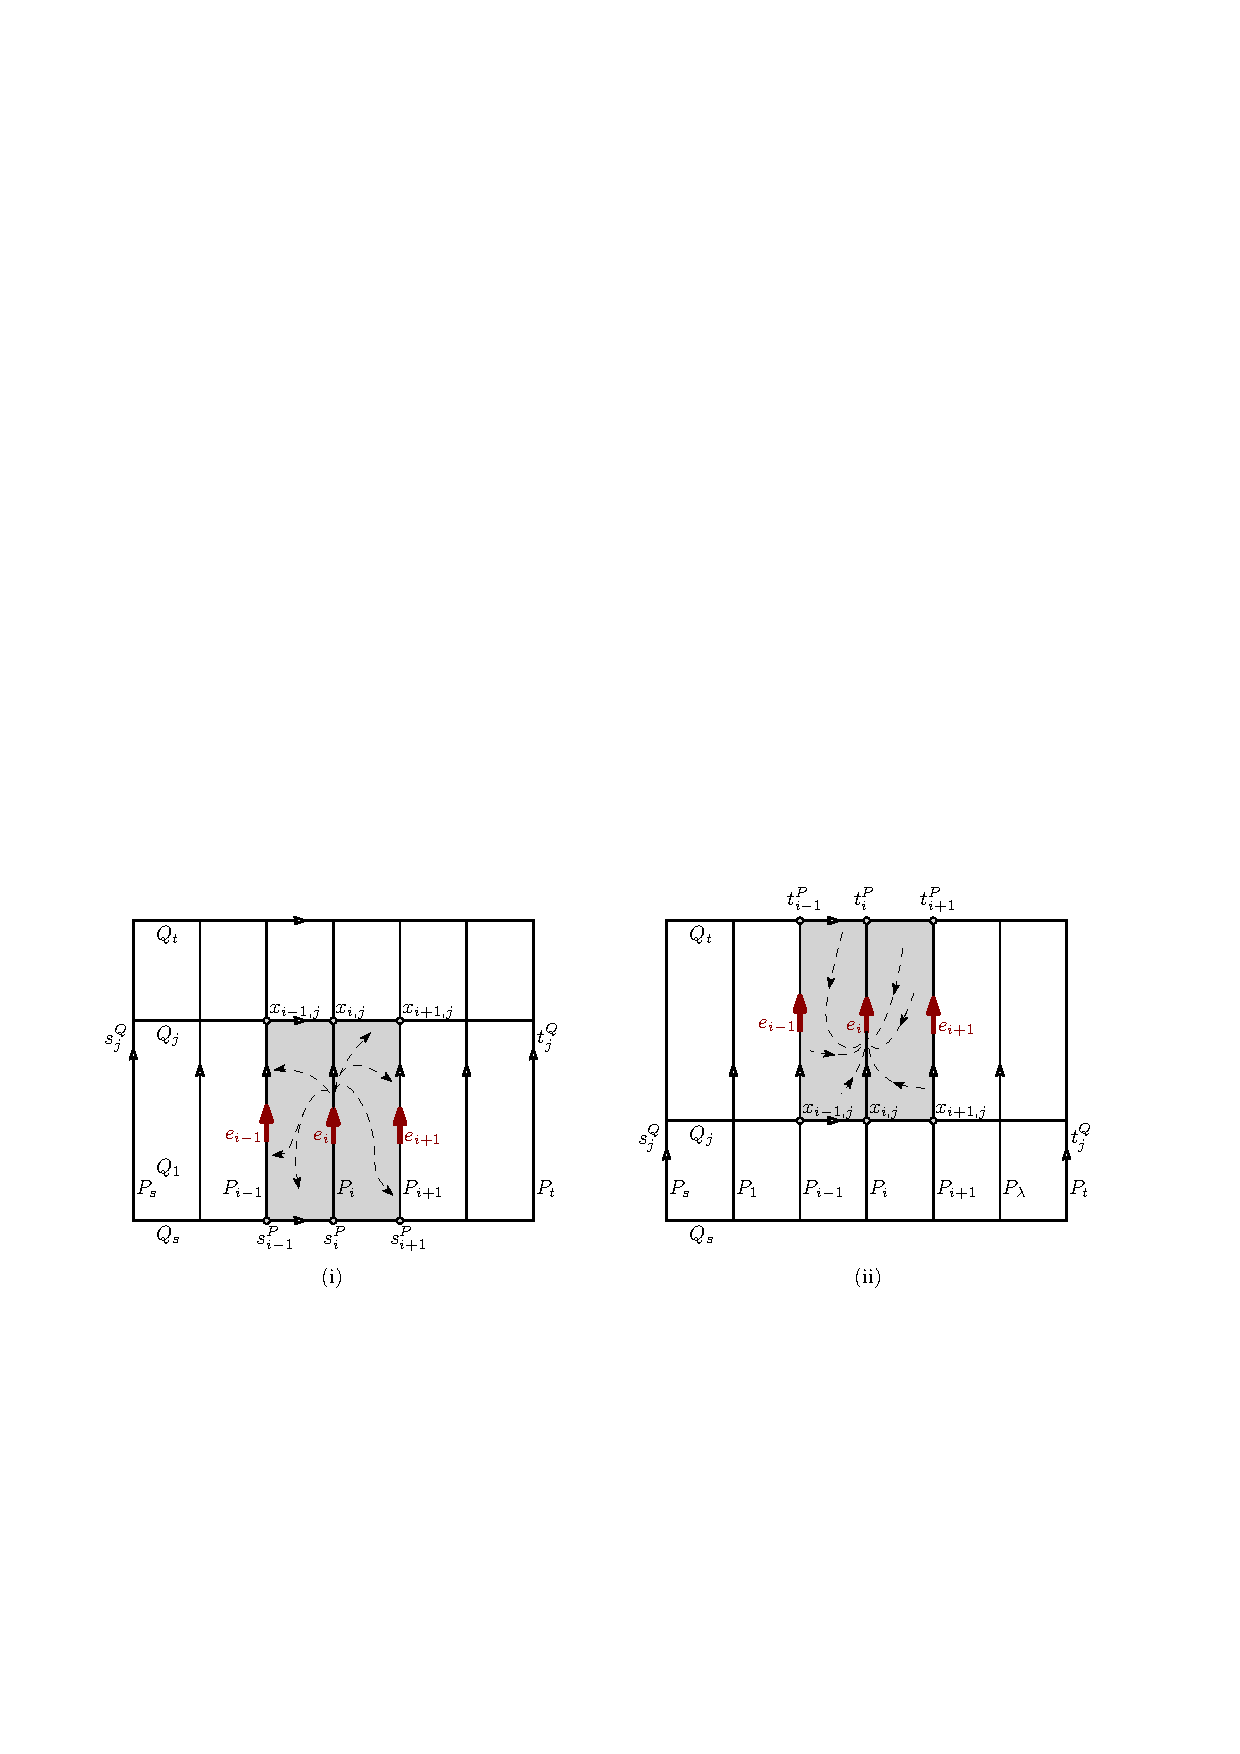
\includegraphics[width=\textwidth]{gridtrap.pdf}
\caption{(i) The demand path $P_d$ is trapped in the shaded region after passing through $e_i$, as entering its boundary is not possible. (ii) The demand path $P_d$ cannot exit the boundary of the shaded region before it passes through $e_i$.}\label{fig:gridtrap}
\end{figure}

\paragraph*{Case 2.} Edge $e_i$ comes after $x_{i,j}$ on $P_i$.
Then $e_i$ is inside the bounded region of the non-directed cycle
\[C'=  x_{i-1,j} \xrightarrow{Q_j} x_{i+1,j} \xleftarrow{P_{i+1}} t^P_{i+1} \xleftarrow{Q_t} s^P_{i-1} \xleftarrow{P_{i-1}} x_{i-1,j}.\]
We claim that after $P_d$ exits $C'$, it cannot pass through $e_i$.
The case can be handled analogously to Case 1: If $P_d$ exits from $Q_j[x_{i-1,j},x_{i+1,j}]$, $Q^t[t^P_i,t^P_{i+1}]$, or $P_{i+1}$ after $e_{i+1}$, then it creates a closed walk, contradicting acyclicity.
Exiting at vertex $x$ of $P_{i+1}$ before $e_{i+1}$ contradicts the essentiality of $e_{i+1}$ for $P_{i+1}$, as $P_{i+1}[x,t^P_{i+1}]$ can be exchanged with $x \xrightarrow{P_d} \head(e_i) \xrightarrow{P_i} t^P_i \xrightarrow{Q_t} t^P_{i+1}$. Exiting from vertex $x$ of $P^\#:=x_{i-1,j} \xrightarrow{P_{i-1}} t^P_{i-1} \xrightarrow{Q_t} t^P_i$ contradicts essentiality of $e_i$ for $P^{ex}_i$, as $P^{ex}_i[u^P_i,t^P_i]$ can be exchanged with $u^P_i \xrightarrow{P_d} x \xrightarrow{P^\#} t^P_i$. \\

The non-existence of a demand $u^Q_ju^P_i$ can be proven as above by exchanging the role of $P_i$ and $Q_j$. If a demand $v^P_iv^Q_j$ could exist, then in the reversed orientation graph it would be a valid demand $u^P_iu^Q_j$, contradicting the above arguments. The non-existence of demands of the form $v^Q_jv^P_i$ then follows by exchanging the role of $P_i$ and $Q_j$ again. This concludes the proof.
\end{proof}

We are now ready to prove the Structure Theorem (Theorem~\ref{thm:maintechnical}).

\begin{proof}[Proof of Theorem~\ref{thm:maintechnical}]
Suppose that $\calD$ is not $c$-bounded, that is, for any positive real number~$\gamma$, there exists an instance $(G_\gamma,T_\gamma,D_\gamma)$ of \Dsn and an optimum solution $H:=H_\gamma$ such that the total branch degree of $H$ is more than $\gamma k$, where $k = |T_\gamma|$.

We say that a quantity $\mu$ is $\gamma$-tied if it can be lower bounded by $\mu>f(\gamma)$ where $\lim_{\gamma \rightarrow \infty} f(\gamma)=\infty$. We need to show that $H$ contains a tough pair whose size is $\gamma$-tied. This implies that we can find a sequence of patterns that have tough pairs whose size goes to infinity. We can use vertex identifications in these patterns on the tough pairs to get patterns with $t$-tough pairs for all positive integers $t$.

As discussed in the beginning of Section~\ref{sec:skeleton}, we may assume without loss of generality that $H$ is acyclic, weakly connected, and the vertices of $H$ have undirected degree at least $3$.

Note that if for each face $\calF$ of $\Skel$ we have that $H\setminus \inter \calF$ fails at most $\kappa$ demands for some absolute constant $\kappa$, then each $H^\calF$ has total branch degree at most $O(\kappa^2)k$ by Lemma~\ref{lem:cbound_face_to_full}, thus we have a face $\calF$ where $H\setminus \inter \calF$ fails at least $\kappa=\Omega(\gamma^{1/2})$ demands. We set $L=\lfloor \kappa^{1/3}\rfloor =\Omega(\gamma^{1/6})$ (in particular, both $\kappa$ and $L$ are  $\gamma$-tied). Now we invoke Lemma~\ref{lem:findgrid}, which gives us a grid structure of size $\lambda=\Omega(L)$, i.e., a grid structure whose size is $\gamma$-tied. Finally, we use Lemma~\ref{lem:gridsarehard} on this grid: we get a $(\lambda-2)$-tough pair. Since $\lambda$ is $\gamma$-tied, this concludes the proof.
\end{proof}